%%%%%%%%%%%%%%%%%%%%%%%%%%%%%%%%%%%%%%%%%
% FRI Data Science_report LaTeX Template
% Version 1.0 (28/1/2020)
% 
% Jure Demšar (jure.demsar@fri.uni-lj.si)
%
% Based on MicromouseSymp article template by:
% Mathias Legrand (legrand.mathias@gmail.com) 
% With extensive modifications by:
% Antonio Valente (antonio.luis.valente@gmail.com)
%
% License:
% CC BY-NC-SA 3.0 (http://creativecommons.org/licenses/by-nc-sa/3.0/)
%
%%%%%%%%%%%%%%%%%%%%%%%%%%%%%%%%%%%%%%%%%


%----------------------------------------------------------------------------------------
%	PACKAGES AND OTHER DOCUMENT CONFIGURATIONS
%----------------------------------------------------------------------------------------
\documentclass[fleqn,moreauthors,10pt]{ds_report}
\usepackage[english]{babel}

\graphicspath{{fig/}}




%----------------------------------------------------------------------------------------
%	ARTICLE INFORMATION
%----------------------------------------------------------------------------------------

% Header
\JournalInfo{FRI Natural language processing course 2021}

% Interim or final report
\Archive{Project report} 
%\Archive{Final report} 

% Article title
\PaperTitle{Offensive language exploratory analysis} 

% Authors (student competitors) and their info
\Authors{Matic Fučka, Anže Alič and Aljaž M. Eržen}

% Advisors
\affiliation{\textit{Advisors: Slavko Žitnik}}

% Keywords
\Keywords{Natural language processing, statistics, hate speech, clustering}
\newcommand{\keywordname}{Keywords}


%----------------------------------------------------------------------------------------
%	ABSTRACT
%----------------------------------------------------------------------------------------

\Abstract{
Offensive language is wide-spread over the internet and other mediums, but we have little insight into it's usage. In this work, we explore how different labels of hate speech relate to each other. We first construct a merged corpus of different datasets and then use various statistical and machine learning methods to find most important words, word and sentence embeddings with clustering and relationships between the classes of hate speech. We find a few distinctive clusters such as ``political harassment'' and describe negative consequences of corpus merging.
}

%----------------------------------------------------------------------------------------

\begin{document}

% Makes all text pages the same height
\flushbottom 

% Print the title and abstract box
\maketitle 

% Removes page numbering from the first page
\thispagestyle{empty} 

%----------------------------------------------------------------------------------------
%	ARTICLE CONTENTS
%----------------------------------------------------------------------------------------

\section*{Introduction}
Different media platforms have different definitions of offensive language and this variation is even higher between different cultures and social classes. The main objective of this assignment is to identify common patters in different classes of hateful speech and to give a better understanding of the relationships between them. 

First we constructed a dataset of hate speech with 20 sentiment labels with the use of different hate speech datasets. They included text which were qualified under different subareas of hate speech by various researchers in the field. We then preprocessed and stemmed the corpus.

After the construction of the dataset we tackled the problem of analysis by extracting the most important words for each label given to us by using some traditional natural language processing (NLP), such as TF-IDF and n-grams, some statistical methods, such as Pearson $\chi^2$ test, some non-contextual neural methods, such as FastText and Word2Vec, and contextual neural methods, such as Bert and Elmo.

With the extracted words we headed onto the calculation of different embeddings for these words or texts. Once we got the embeddings we tried different clustering methods such as PCA, t-SNE, and LDA to group these embeddings. We also discussed the results of the approaches that yielded some useful information.


%------------------------------------------------

\section*{Datasets and literature overview}

For the sake of this assignment we used 7 different datasets with various labels. 

Chung et al. \cite{16_facebook} proposed a large multilingual(English, French and Italian) dataset, which has been produced by operators from various NGOs that deal with a common field. Besides hate speech they also produced non-hate speech that provided a counter-narrative. They also mostly dealt with hate towards Muslims and some other religious groups.

Ousidhom et al. \cite{20_twitter} have produced a dataset in three different languages: English, French and Arabic. They collected 13,000 potentially derogatory tweets and used Amazon Mechanical Turk to label them. As they thought that for investigation of the motivation and behavior of user that use such language a binary classification does not suffice, they added several labels to their tweets. They added whether the text is direct or indirect, whether it is offensive, disrespectful, hateful, fearful, abusive or normal, whether it discriminates towards individuals or towards a group of people and towards which group and they also labeled the annotators feelings about the content.

Rezvan et al. \cite{32_twitter} have produced a dataset of 24189 tweets which have been labeled by the type of harassment (sexual, racial, appearance-related, intellectual and political). They've collected this tweets with the help of the keywords for each subsection compiled by several online resources. Besides harassment they have labeled this data as cyberbullying a few times throughout the paper.

Cachola et al. \cite{vulgar-twitter} have collected a dataset containing vulgar tweets. As before they collected this dataset by collecting all of the last 3200 tweets produced by 4,132 user with known socio-demographic traits that contained at least one of the vulgar keywords compiled from online resources. After some preprocessing and labeling they ended with 6718 tweets that were indeed vulgar.

Mandl et at. \cite{25_twitter} created a dataset of tweets collected by various heuristics to find typical Hate Speech. With these tweets and Facebook posts they also downloaded the latest tweets of these users to increase variety. Then they labeled this data using online judge systems by various juniors in each language. With the usage of such a system they also question the accuracy of their dataset.

The Conversation AI team \cite{kaggle-jigsaw} have proposed on online competition on Kaggle to improve current models that classify toxic posts from Wikipedia comments. These comments have been labeled by human raters for toxic behaviour. It contains of 41335 comments with insult, none, obscene, threat, identity hate, sever toxic and toxic labels.

Chandrasekharan et al. \cite{zenodo} have created a dataset of removed comments from 100 different communities on Reddit. These comments were removed by moderators due to breaking some of the communities rules. With these justifications they labeled around 40,000 comments and split them into several datasets. We used the dataset that contained comments that were determined to be slurs and it contained 5059 such comments.


\section*{Methods}

\subsection*{Corpus merging}

Overall, the 7 datasets together include 19 different labels for hate speech types and a ``not hate speech'' label. Collections sources include Twitter \cite{20_twitter, 32_twitter, vulgar-twitter, 25_twitter}, Facebook \cite{16_facebook}, Wikipedia comments \cite{kaggle-jigsaw} and Reddit \cite{zenodo}. Which dataset contained which labels and how many of them can be seen in Table~\ref{tab:sentiment-source}.
% abusive appearance_harassment disrespectful fearful hateful homophobic insult intelligence_harassment misogynistic obscene offensive political_harassment profanity racist severe_toxic sexual_harassment threat toxic vulgar none
It should be noted that some labels were present only in one dataset and some datasets had all documents labeled with a single label. Documents of one dataset were labeled with multiple labels, which we solved by mapping each of the documents into multiple replicas where each of them was labeled with one of initial labels (e.g. document labeled as \texttt{fearful\_abusive\_hateful} was replicated into 3 documents with labels \texttt{fearful}, \texttt{abusive}, and \texttt{hateful}).

Some datasets did not label \textit{type of hate speech} but labeled sentiment, directness, target, group or some other property. From this we interpolated our \textit{type of hate speech} using best effort approximations. For example, we labeled \texttt{hostile} sentiment with target \texttt{women} as \texttt{misogynistic} and target \texttt{sexual\_orientation} with \texttt{homophobic}. This relabeling is not ideal due to gap between the meanings, which is why we interpolated only labels that were not found anywhere else, so there would not be clash between meanings of a single label.

Our process of merging datasets is not ideal because replicating multi-label documents introduces high correlation between labels from this dataset. Also, if labels are provided by only one dataset, we are essentially only comparing the biases of the datasets. This bias is composed of annotator's bias in interpretation of some \textit{type of hate speech} (which is what we are after) and other biases such as collection source of the dataset or preprocessing techniques. This is why results of our analysis cannot necessarily confirm correlation between labels as correlations between \textit{types of hate speech}, because it may be caused by other biases.

\subsection*{Data preprocessing}
Text in our corpus is mostly from online sources such as Twitter, which is why we had to remove emojis, tags etc. We first replaced emojis with corresponding words (e.g. replace fire emoji with word ¨fire"). Than we used special Twitter tokenizer to tokenize text into tokens. We removed tokens that correspond to urls, mentions, unknown emojis or hashtags. In the end, we stemmed each token with Snowball stemmer.

%\subsection*{Pearson $\chi^2$ test}

%The Pearson $\chi^2$ test is an statistical hypothesis, which determines whether there is a statistically significance between the expected and the observed frequencies. If we define $E_G(w)$ the expected frequency of the word $w$ in some general corpus $G$ and $O_R(w)$ the observed frequency in specific corpus $R$ then the value of the Pearson $\chi^2$ test for word w (which we dub $P_R(w)$) is as follows:
% \begin{equation}
%     P_R(w) = \frac{(E_G(w)-O_R(w))^2}{E_G(w)}
% \end{equation}
% If the value of the Pearson $\chi^2$ test $P_R(w)$ exceeds 3.84 for some word $w$ in a specific corpus $R$ then we are able to say with a 95\% certainty that the word $w$ is statistically significant for the corpus $R$.

% \subsection*{FastText}
% FastText is a non-contextual neural model for learning word embeddings in an either supervised or an unsupervised manner. It is an extension of the word2vec model but instead of learning the vectors for words directly it learns each word as an n-gram of characters. This helps the model to understand prefixes and suffixes. Once the word is represented using n-gram characters a skip-gram model is trained to learn the embeddings. The biggest improvement of fastText over GloVe and word2vec is that you are able to get the embeddings of words that were not present during training.
%------------------------------------------------

\section*{Experiments}

\subsection*{Important words retrieval}

We retrieved most important words in a couple of different ways. First we extracted most common 1-grams, 2-grams and 3-grams for each label. The results were mostly as expected with "retard" and "fuck" being one of the most common 1-grams for a quite high number of labels. Another interesting finding is that there is quite a lot of swear words in non-hate speech, which was quite the opposite of our expectations. We also checked which labels share the most most common words. What we noticed is that fearful, offensive, abusive and disrespectful have a lot of words, which are predominantly swears, in common. Another such cluster is toxic, obscene and insult. Other labels tend to have different words. When we looked into it we noticed these cluster have words that do make sense, so we are able to conclude that these clusters tend to cover similar topics.

Then we extracted the most statistically significant words for each label. Only the labels related to some sort of harassment had statistically significant words. Appearance harassment had "fatass", political harassment had "twatwaffle", and sexual harassment had "camel", "toe", "grab", "sporty", "ssi" (special sex interest) and "skullfuck". Even though we saw that each label tends to have its own most common words, there is few statistically significant words.

%% TFIDF

\begin{table}[h]
    \centering
    \begin{tabular}{ll}
        \toprule
                      Label &         3 most important words \\
        \midrule
                        abusive &      shithol, ching, chong \\
          appearance harassment &          fatass, skank, rt \\
                  disrespectful &      shithol, ching, chong \\
                        fearful &      shithol, ching, chong \\
                        hateful &        shithol, icc, chong \\
                     homophobic &            dyke, game, nit \\
                         insult &       wikipedia, jew, page \\
        intelligence harassment &     fucktard, rt, shithead \\
                   misogynistic &     feminazi, mongi, chong \\
                           none &    articl, page, wikipedia \\
                        obscene &      wikipedia, page, edit \\
                      offensive &      shithol, ching, chong \\
           political harassment & islam, religion, twatwaffl \\
                      profanity &        icc, doctor, mamata \\
                         racist &     paki, beaner, sandnigg \\
              sexual harassment &           camel, toe, grab \\
                           slur &           reddit, mod, com \\
                         threat &         0ll, supertr, wale \\
                          toxic &      wikipedia, page, edit \\
                         vulgar &              damn, amp, ho \\
        \bottomrule
        \end{tabular}
    \label{tab:tf_idf}
    \caption{3 most important words by the TF-IDF (with parameter max df=0.8, max features=200000 and min df=0.2) method for each label}
\end{table}

Similarly, we used TF-IDF to extracted the most common words for each label. For the majority of the labels, we got good results as seen in table \ref{tab:tf_idf}. For example, for racist we get "paki", for disrespectful "shithol", "ching" and "chong". But there are also some labels such as toxic where the most important word is "wikipedia", which does not make sense. 

\subsection*{Interlabel exploration}

After we extracted the most important words for each label, we decided to check if there are similarities between texts with the same labels from different datasets. We had 3 such labels: Hateful, Offensive and Political harassment. For each source of the label we checked the most common 1,2 and 3-grams, the most important words according to the Pearson $\chi^2$ test and the most important words according to TF-IDF. For TF-IDF we used 1-grams, maximal dictionary frequence of 0.8, minimal dictionary frequency of 0.2 and english stopwords.

What we found out is that these datasets heavily differ from one another and there is little correlation between the labels.

\subsection*{Label grouping}
We grouped our data using hierarchical clustering for different ways of important words extraction (n-grams and TF-IDF), then we used different types of embeddings on these words (TF-IDF, trained and pretrained FastText, Word2Vec) and clustered it different types of clusterings or dimension reductionality (PCA, LDA, MDS, T-SNE). In the following section we will discuss in detail the approaches that yielded some useful information.  

Number of common word extracted with TF-IDF (with parameter max df=0.8, max features=200000 and min df=0.2) can be seen in figure \ref{fig:common_tfidf}. We can observe that labels abusive, disrespectful, fearful, hateful, misogynistic, and offensive are very similar. There are other similar pairs of labels such as intelligence and political harassment, appearance and sexual harassment.
\begin{figure}
    \centering
    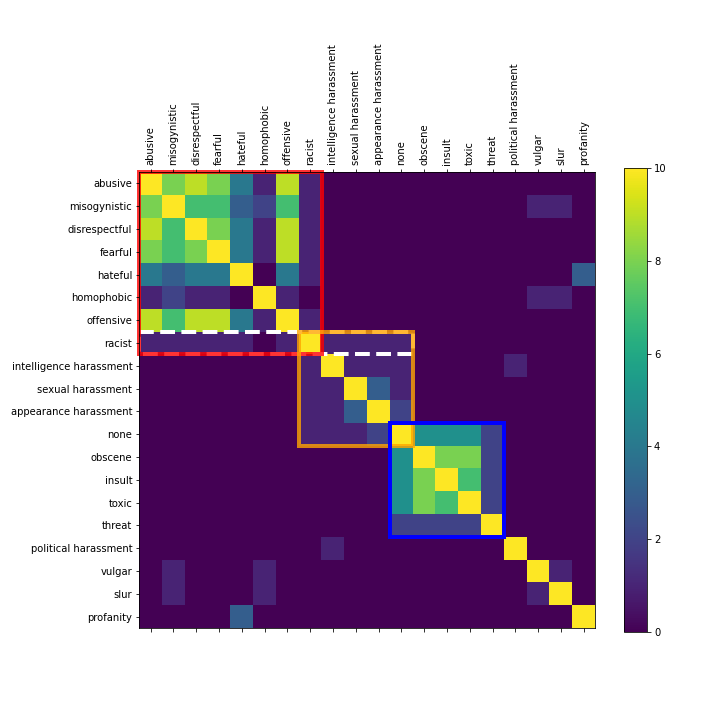
\includegraphics[width=\columnwidth]{fig/heatmap_of_common_words.png}
    \caption{The number of common words extracted with TF-IDF(with parameter max df=0.8, max features=200000 and min df=0.2). We have three main distinct clusters. For red cluster common words are "shithol", "ching", "chong" etc. For blue one "wikipedia","page" etc. Another interesting observation is that racist have common words with two clusters. This means that racist speech(white) contains other categories such as offensive, abusive, appearance harassment.}
    \label{fig:common_tfidf}
\end{figure}
We come to the same conclusion if we use hierarchical clustering. The dendrogram can be seen in figure \ref{fig:hierarchical_tfidf}.
\begin{figure}
    \centering
    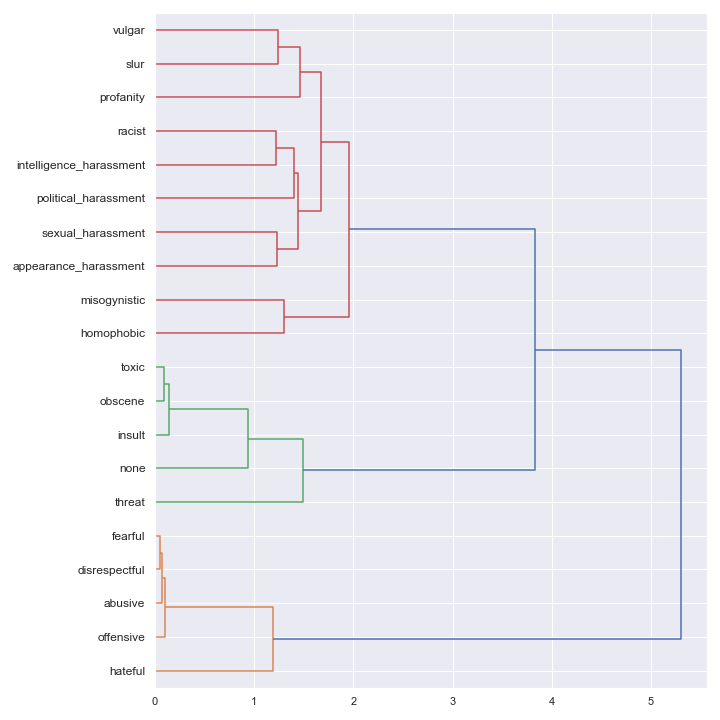
\includegraphics[width=\columnwidth]{fig/tf-idf_cluster.png}
    \caption{30 important words extracted for each label with TF-IDF(with parameter max df=0.8, max features=200000 and min df=0.2). Labels cluster using TF-IDF coefficients.}
    \label{fig:hierarchical_tfidf}
\end{figure}

We used word embeddings from TF-IDF(with parameter max df=0.8, max features=200000 and min df=0.2) coefficients for the most important words for each label according to TF-IDF. 2D projection can be seen in figure \ref{fig:tfidf_embedding}.
\begin{figure}
    \centering
    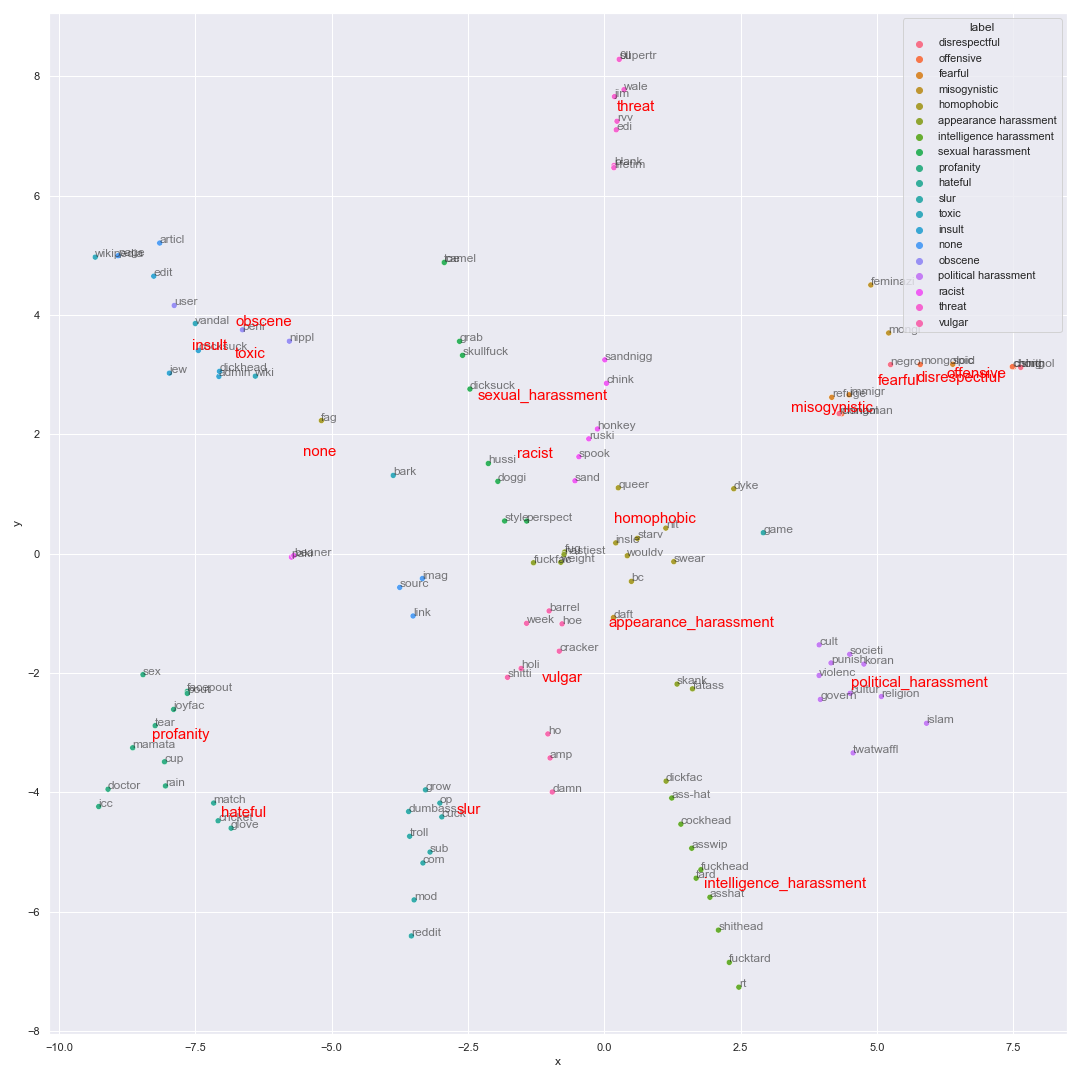
\includegraphics[width=\columnwidth]{fig/TSNE-tfidf.png}%[width=\columnwidth]
    \caption{Important words embedded with t-SNE using TF-IDF(with parameter max df=0.8, max features=200000 and min df=0.2) coefficients.}
    \label{fig:tfidf_embedding}
\end{figure}
We can observe that appearance and intellectual harassment are in the same cluster. The same is with obscene and insult. But there are also clusters that stands for it own such as slur, threat, profanity and threat.

To project data to 2D we also used LDA (Linear Discriminant Analysis), which does not only use embeddings but also the words label. We used only the words with one label out of the most important ones. The projection can be seen in figure \ref{fig:fasttext_LDA}.
\begin{figure}
    \centering
    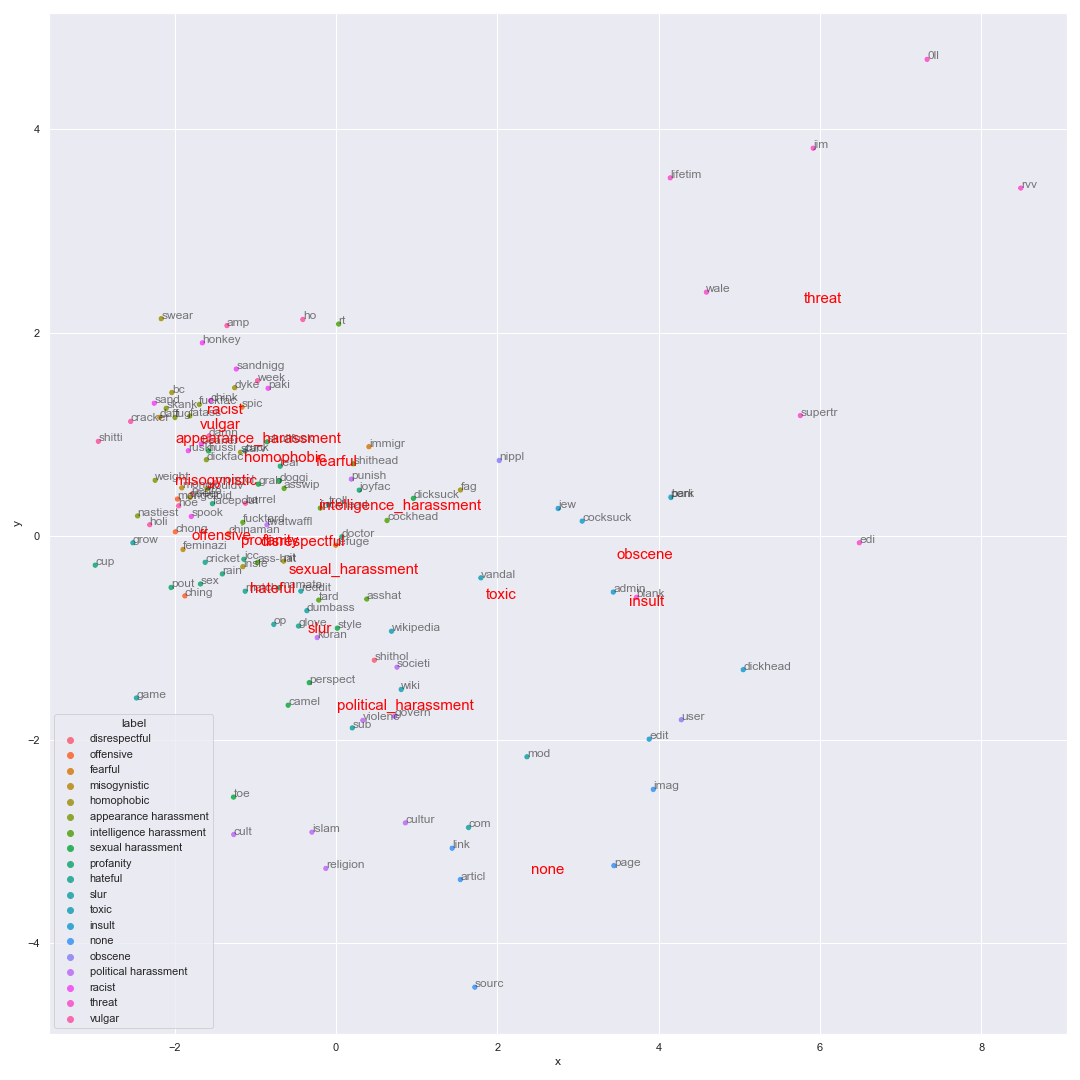
\includegraphics[width=\columnwidth]{fig/LDA-fasttext.png}%[width=\columnwidth]
    \caption{Important words embedded with FastText(vector size is 16 and window is of size 3) and projected using LDA.}
    \label{fig:fasttext_LDA}
\end{figure}
Most important observation we can make is that the label none is separable from all of the other labels, which is to be expected. Political harassment seems differs from other labels, as it is a bit further away from the central cluster. We would probably tend to say the same if we had to judge it subjectively. Racist, vulgar and appearance harassment are very similar to each other with similar words such as ``dickface".

% Word2Vec
We trained our own Word2Vec model and also use some pretrained(such as word2vec-google-news-300) ones, but the embeddings were not informative. We were not able to recognize any clusters or structure in the data. The reason is probably the fact that our corpus is not large enough, to make good estimate of the weights. Another problem is that most of data are tweets and sentences are semantically poor. 

%FastText
When we used the FastText model we trained it on the whole corpus but took only the labels embeddings, and reduced its dimensionality with PCA and plotted it on a 2D plane. The results are shown on Figure~\ref{fig:fasttextpca}. From the figure a few clusters can be seen. As we can see we have a cluster with vulgarity, profanity, slur and fearful, which mostly makes sense as the labels tend to have a similar meaning. Another cluster is none and abusive, which does not make sense. We could explain this only by assuming that this embedding shows us some of the underlying bias of our corpus (at least for this two labels), In the centre of the coordinate system we have a slightly bigger cluster, with different types of harassment, offensive, disrespectful, hateful and misogynistic. The common line with this labels is that they tend to focus on the "outside" or the "inside" properties of the victim. Homophobic, racist, insult and threat are laying outside of these clusters.

\begin{figure}
    \centering
    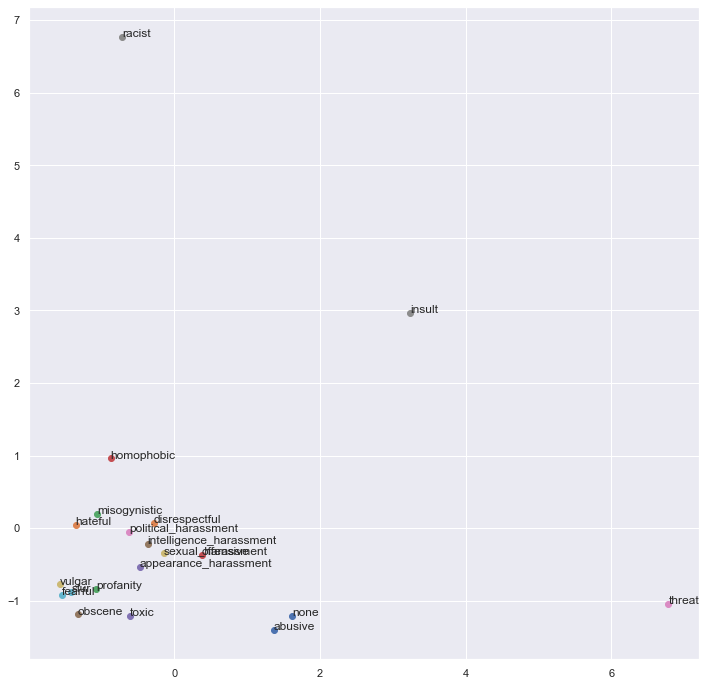
\includegraphics[width=0.7\columnwidth]{fig/fastText_PCA.png}
    \caption{PCA decomposition of FastText embeddings for each label. FastText was trained on the merged dataset. It had a vector size of 20, window size of 3 and it was trained on each word of the corpus(min count = 1).}
    \label{fig:fasttextpca}
\end{figure}

%------------------------------------------------
FastText was also used to find most similar words to labels. Embedding can be seen in figure \ref{fig:fasttext_embedding}.
\begin{figure*}
    \centering
    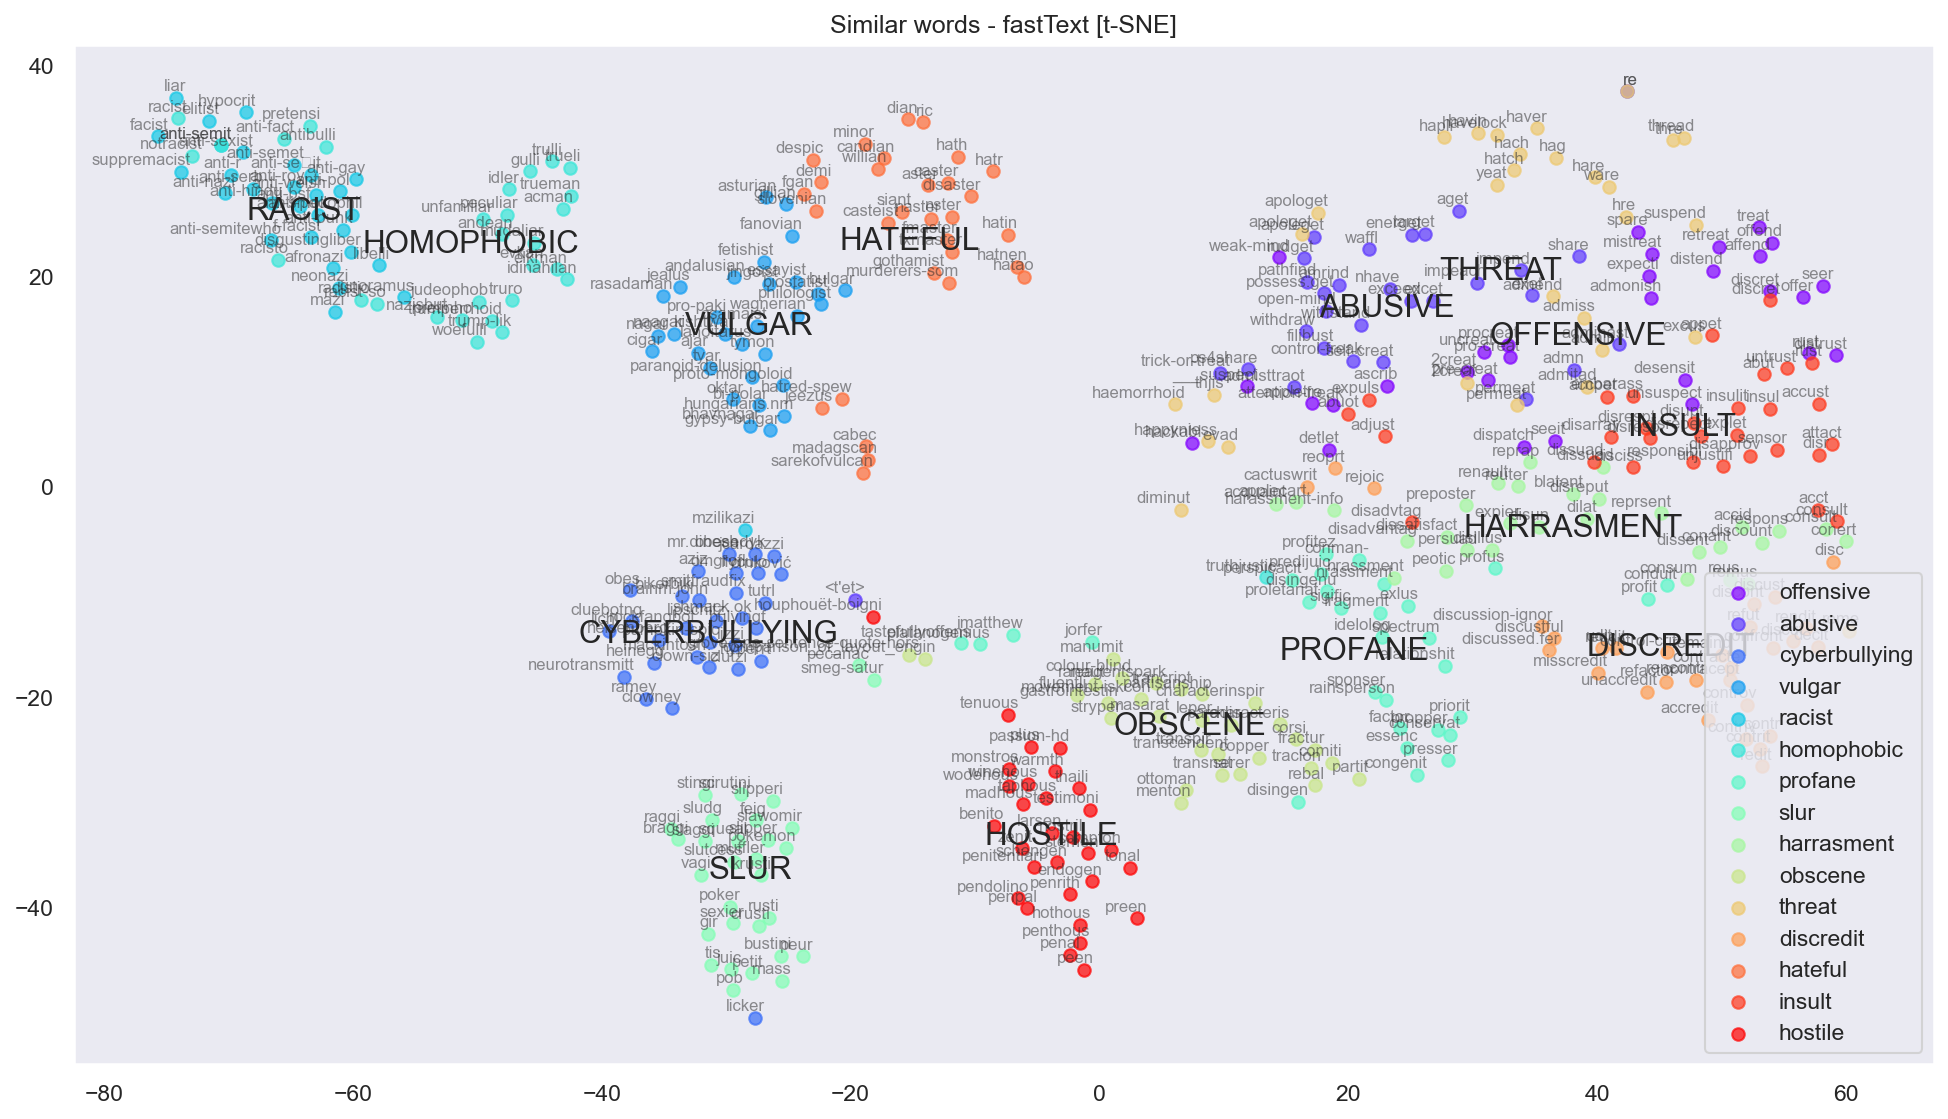
\includegraphics[width=\textwidth]{fig/SimilarWords - fastText - t-SNE.png}
    \caption{Most similar words retrieved by FastText(vector size is 16 and window is of size 3).}
    \label{fig:fasttext_embedding}
\end{figure*}
For some labels we get exquisite results. For instance, with the label racist we get that some of the most similar words are "neonazi","anti-semit", "facist" etc. But for many other labels most similar words do not make a lot of sense. Most of the labels are separable from the others and forms compact clusters such as slur, cyberbullying, vulgar, hateful, obscene etc. But there are labels which are very similar. For instance threat, abusive, offensive. For the compact ones we are able to say that most probably these labels cover their own area of swear words.

\subsection*{Deep neural networks}

We have experimented with ELMo \cite{ElmoSemEval} (bi-directional LSTM), which we initialized with pre-trained model, built on ``News on the Web'' corpus. For each of the documents, we computed average over embeddings of each word and preformed dimensionality reduction with PCA and t-SNE. Results did not show significant separation between sentiment classes, but did show a few clusters of mixed classes. It should be noted we did not embed all documents from the dataset, but only random 2000, because even with using a GPU ELMo proccessed only 15 documents per second.

On the other hand, BERT generated better results. At first, we used plain pre-trained BERT to produce embeddings from last hidden state (average over each input token) or from pooled output. Similarly we used PCA and t-SNE, but also did not find significant separation between classes. Then, we constructed a compound model from BERT and two dense layers. The first performs \textit{embedding} of pooled BERT output into 10 units and the second \textit{classifies} them for each of the output labels. After a brief training of the last two layers, the classification accuracy on validation dataset converged to $0.337$, which is significantly better than baseline of random classification with accuracy $\frac{1}{20} = 0.05$. We then evaluated the model on test dataset and used outputs of the first dense layer as an embedding. From figure \ref{fig:bert_tsne} we can see that some of the classes (like political harassment and slur) are clearly separable.

\begin{figure}[h]
    \centering
    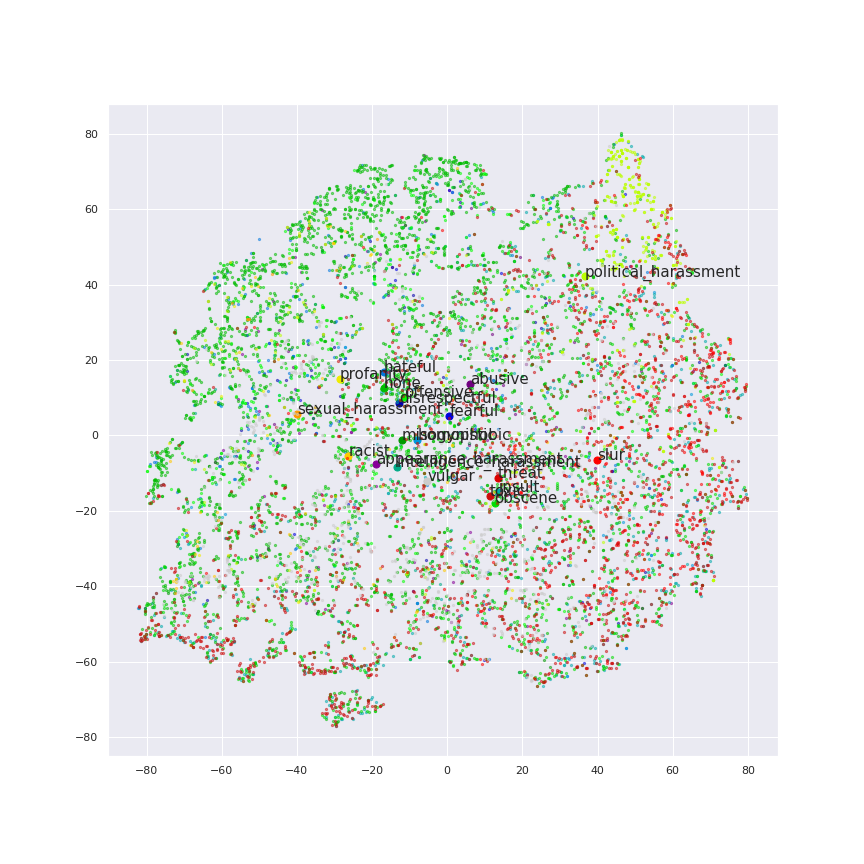
\includegraphics[width=\linewidth]{bert_sent_embed_tsne.png}
    \caption{Visualization of embedding produced with fine-tuned extended BERT model. 10 dimensions were reduced with t-SNE. Pretrained model is accessible at \url{https://huggingface.co/bert-base-cased}.}
    \label{fig:bert_tsne}
\end{figure}

Unfortunately, both of the most separable clusters correspond to classes that originate from single dataset, which suggests that the differences between classes could be attributed to dataset bias. This can be clearly confirmed with figure \ref{fig:bert_tsne_source} which shows same embedding, but visualises source datasets.

\begin{figure}[h]
    \centering
    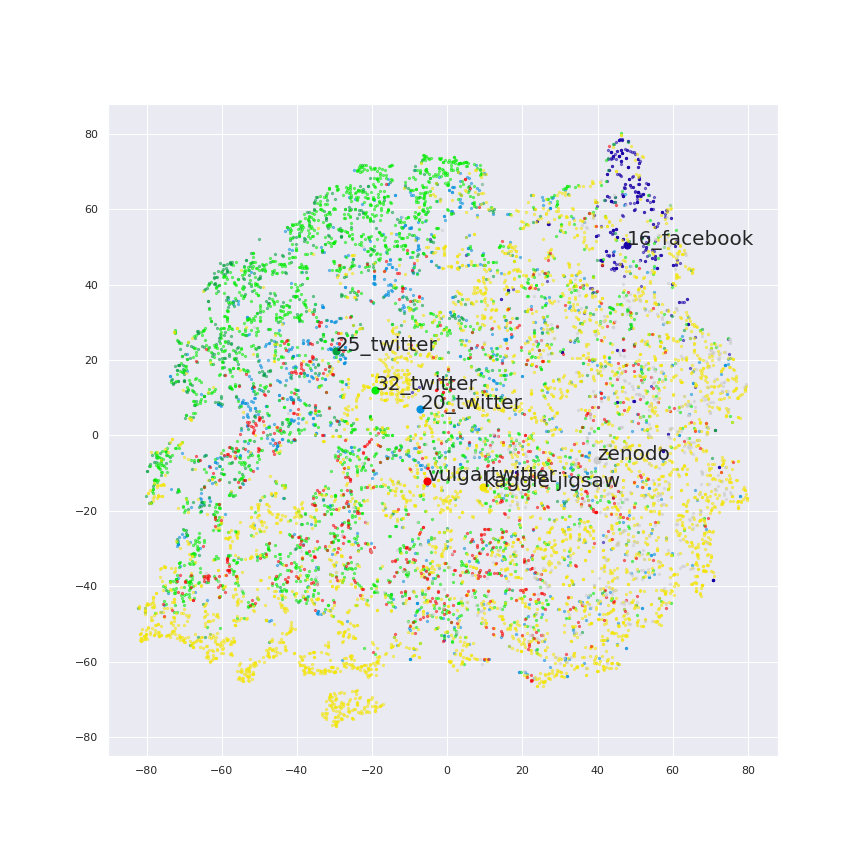
\includegraphics[width=\linewidth]{bert_source_embed_tsne.png}
    \caption{Same embedding as in figure \ref{fig:bert_tsne}, but colored by dataset.}
    \label{fig:bert_tsne_source}
\end{figure}

\section*{Results}

Based on the results of different methods in the previous section we were able to determine a few clusters for labels that are similar based on our dataset. Because results of different methods don't have a consistent way of merging, we combined them by hand, using best effort. Although some of our final clusters might not be consistent with all previous results, we believe that each of them is consistent with majority. These clusters can be seen in Table~\ref{tab:clusters}. 

Given our results and the fact that authors of the source datasets provided little semantic information about the labels, we are unable to draw more conclusions about relationships between these clusters.

\begin{table}[h]
    \centering
    \begin{tabular}{ll}
        \toprule
        Cluster \# & Labels \\
        \toprule
        1 & \parbox[t]{5cm}{appearance\_harassment, fearful, homophobic, racist, vulgar} \\
        2 & disrespectful, offensive, profanity \\
        3 & insult, obscene, toxic \\
        4 & hateful, misogynistic, sexual\_harassment \\
        5 & cyberbullying \\
        6 & discredit \\
        7 & intelectual\_harassment \\
        8 & political\_harassment \\
        9 & slur \\
        10 & threat \\
        \toprule
    \end{tabular}
    \caption{Label clusters based on our results}
    \label{tab:clusters}
\end{table}

\section*{Conclusion}

Even though we were able to identify label clusters, we are not highly confident in the results. Primarily, the reason is our merged corpus. As described in \textit{Interlabel exploration} section, variation within labeled classes is generally higher than variation between the classes. This is caused by the fact that datasets contributing to a single label differ significantly.  

As a consequence, we cannot confirm any inter-label hypothesis based on results found on the merged corpus. This is because these results may be caused by variation among source datasets and their data collection methods. We can confirm this with the fact, that a large portion of label clustering results is highly correlated with dataset clustering (see TF-IDF important words, BERT embedding).

In summary, dataset merging introduces high variability between source datasets, which can overshadow variation you are trying to measure. We suspect that this would hold in general, except in some highly specific in-domain cases. That is; when data collection methods are similar for all datasets, actual sources (i.e. online forum, news articles) are picked more narrowly and are more similar to each other.

Also, this invokes a following question: how would results of studies performed a dataset change if we were to evaluate the same study on a different dataset? If we know that inter-dataset variance is high, probability that the results would significantly change may be high. If this is true, many of the conclusions drawn with similar datasets may not hold and we have to rethink our standards for data collection from online sources.

\begin{table*}[]
\centering
\begin{tabular}{l|rrrrrrr|r}
          & & & & Dataset & & & & \\
Sentiment & 16 fcbk & 20 twtr & 25 twtr & 32 twtr & wikipedia & vulgar twtr & reddit & total \\
\midrule
  %\hline
  abusive &   0 & 671 &   0 &   0 &   0 &   0 &   0                   & 671   \\ 
  appearance\_harassment &   0 &   0 &   0 & 677 &   0 &   0 &   0    & 677   \\ 
  disrespectful &   0 & 782 &   0 &   0 &   0 &   0 &   0             & 782   \\ 
  fearful &   0 & 562 &   0 &   0 &   0 &   0 &   0                   & 562   \\ 
  hateful &   0 & 1278 & 1267 &   0 &   0 &   0 &   0                 & 2545  \\ 
  homophobic &   0 & 845 &   0 &   0 &   0 &   0 &   0                & 845   \\ 
  insult &   0 &   0 &   0 &   0 & 7877 &   0 &   0                   & 7877  \\ 
  intelligence\_harassment &   0 &   0 &   0 & 810 &   0 &   0 &   0  & 1360  \\ 
  misogynistic &   0 & 1360 &   0 &   0 &   0 &   0 &   0             & 33157 \\ 
  none &   0 &   0 & 4456 & 21059 & 7642 &   0 &   0                  & 810   \\ 
  obscene &   0 &   0 &   0 &   0 & 8449 &   0 &   0                  & 8449  \\ 
  offensive &   0 & 4020 & 522 &   0 &   0 &   0 &   0                & 4542  \\ 
  political\_harassment & 3864 &   0 &   0 & 698 &   0 &   0 &   0    & 4562  \\ 
  profanity &   0 &   0 & 760 &   0 &   0 &   0 &   0                 & 760   \\ 
  racist &   0 &   0 &   0 & 702 &   0 &   0 &   0                    & 702   \\ 
  sexual\_harassment &   0 &   0 &   0 & 229 &   0 &   0 &   0        & 229   \\ 
  slur &   0 &   0 &   0 &   0 &   0 &   0 & 5059                     & 5059  \\ 
  threat &   0 &   0 &   0 &   0 & 478 &   0 &   0                    & 478   \\ 
  toxic &   0 &   0 &   0 &   0 & 16889 &   0 &   0                   & 16889 \\ 
  vulgar &   0 &   0 &   0 &   0 &   0 & 6718 &   0                   & 6718  \\ 
   %\hline
  \bottomrule
  total & 3864 & 9518 & 7005 & 24175 & 41335 & 6718 & 5059            & 97674 \\
\end{tabular}
\caption{Number of documents for different sentiments and sources. Prefix numbers of sources are indexes from \url{https://hatespeechdata.com/}}
\label{tab:sentiment-source}
\end{table*}

\newpage
%----------------------------------------------------------------------------------------
%	REFERENCE LIST
%----------------------------------------------------------------------------------------
\bibliographystyle{unsrt}
\bibliography{report}


\end{document}